\documentclass[../../../include/open-logic-section]{subfiles}

\begin{document}

\olfileid{sth}{ordinals}{idea}
\olsection{ક્રમવાચક સંખ્યાનો સામાન્ય ખ્યાલ}

પ્રાકૃતિક સંખ્યાઓને તેમના સામાન્ય ક્રમમાં વિચારો:
\begin{center}
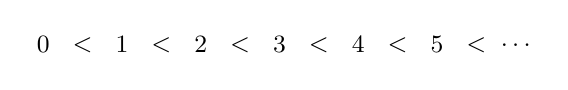
\begin{tikzpicture}
	\foreach \x/\xtext in {0, 1, 2, 3, 4, 5}
	{
		\node (\x a) at (\x, 1) {\small{$\x$}};
		\node (\x a) at (\x.5, 1) {\small{$<$}};
	}
	\node (ldots) at (6, 1) {\small{$\ldots$}};
	\end{tikzpicture}
\end{center}
પરિભાષામાં આપણે આને $\omega$-અનુક્રમ કહીએ છીએ.
ખરેખર, ગણોના પદાનુક્રમના તબક્કાઓની આપણી શરૂઆતની
રચનામાં પણ આ સામાન્ય ક્રમ પ્રતિબિંબિત થાય છે.
પણ હવે ધારો કે $0$ને આ અનુક્રમના અંતે મૂકીએ,
એટલે તે બીજી બધી સંખ્યાઓ પછી આવે:
\begin{center}
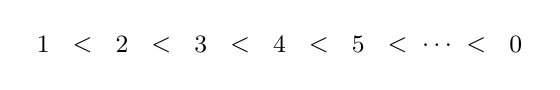
\begin{tikzpicture}
	\foreach \x/\xtext in {1, 2, 3, 4, 5}
	{
		\node (\x a) at (\x, 1) {\small{$\x$}};
		\node (\x a) at (\x.5, 1) {\small{$<$}};
	}
	\node (ldots) at (6, 1) {\small{$\ldots$}};
	\node (bea) at (6.5, 1) {\small{$<$}};
	\node (noa) at (7, 1) {\small{$0$}};
	\end{tikzpicture}
\end{center}
અહીં વસ્તુઓ એ જ છે, પણ તેમનો ક્રમ મૂળભૂત રીતે જુદો
છે: પહેલા ક્રમમાં અંતિમ ઘટક નહોતો; નવા ક્રમમાં છે.
ખરેખર, નવા ક્રમમાં વસ્તુઓનો $\omega$-અનુક્રમ
($1, 2, 3, 4, 5, \ldots$) આવે છે અને પછી બીજી
એક વસ્તુ આવે છે. આ $\omega+1$-અનુક્રમ થશે.

માત્ર આ જ વસ્તુઓથી ક્રમના વધુ પ્રકારો બનાવી શકીએ.
ઉદાહરણ તરીકે, બધી બેકી સંખ્યાઓ (તેમના સ્વાભાવિક
ક્રમમાં), અને પછી બધી એકી સંખ્યાઓ (તેમના સ્વાભાવિક
ક્રમમાં) વિચારો:
\begin{center}
\begin{tikzpicture}
	\node(a1) at (1,1) {\small{$0$}};
	\node(a2) at (1.5,1) {\small{$<$}};
	\node(a3) at (2,1) {\small{$2$}};
	\node(a4) at (2.5,1) {\small{$<$}};
	\node(a5) at (3,1) {\small{$4$}};
	\node(a6) at (3.5,1) {\small{$<$}};
	\node(dots) at (4,1) {\small{$\ldots$}};
	\node(aaoe) at (4.5,1) {\small{$<$}};
	\node(b1) at (5,1) {\small{$1$}};
	\node(b2) at (5.5,1) {\small{$<$}};
	\node(b3) at (6,1) {\small{$3$}};
	\node(b4) at (6.5,1) {\small{$<$}};
	\node(b5) at (7,1) {\small{$\ldots$}};
	\end{tikzpicture}
\end{center}
આ એક $\omega$-અનુક્રમ પછી બીજો $\omega$-અનુક્રમ
છે; એટલે $\omega+\omega$-અનુક્રમ.

આમ આપણે આગળ વધતા રહી શકીએ. પણ \emph{ક્રમો}
વિશેની આ વાતને સમજવાની એક સામાન્ય રીત જોઈએ છે.

\end{document}
